\documentclass[11pt,]{article}
\usepackage{lmodern}
\usepackage{amssymb,amsmath}
\usepackage{ifxetex,ifluatex}
\usepackage{fixltx2e} % provides \textsubscript
\ifnum 0\ifxetex 1\fi\ifluatex 1\fi=0 % if pdftex
  \usepackage[T1]{fontenc}
  \usepackage[utf8]{inputenc}
\else % if luatex or xelatex
  \ifxetex
    \usepackage{mathspec}
  \else
    \usepackage{fontspec}
  \fi
  \defaultfontfeatures{Ligatures=TeX,Scale=MatchLowercase}
\fi
% use upquote if available, for straight quotes in verbatim environments
\IfFileExists{upquote.sty}{\usepackage{upquote}}{}
% use microtype if available
\IfFileExists{microtype.sty}{%
\usepackage{microtype}
\UseMicrotypeSet[protrusion]{basicmath} % disable protrusion for tt fonts
}{}
\usepackage[margin = 1.75in]{geometry}
\usepackage{hyperref}
\PassOptionsToPackage{usenames,dvipsnames}{color} % color is loaded by hyperref
\hypersetup{unicode=true,
            pdftitle={Graphics with ggplot()},
            pdfauthor={Abhinav Anand},
            colorlinks=true,
            linkcolor=blue,
            citecolor=magenta,
            urlcolor=red,
            breaklinks=true}
\urlstyle{same}  % don't use monospace font for urls
\usepackage{color}
\usepackage{fancyvrb}
\newcommand{\VerbBar}{|}
\newcommand{\VERB}{\Verb[commandchars=\\\{\}]}
\DefineVerbatimEnvironment{Highlighting}{Verbatim}{commandchars=\\\{\}}
% Add ',fontsize=\small' for more characters per line
\usepackage{framed}
\definecolor{shadecolor}{RGB}{248,248,248}
\newenvironment{Shaded}{\begin{snugshade}}{\end{snugshade}}
\newcommand{\KeywordTok}[1]{\textcolor[rgb]{0.13,0.29,0.53}{\textbf{#1}}}
\newcommand{\DataTypeTok}[1]{\textcolor[rgb]{0.13,0.29,0.53}{#1}}
\newcommand{\DecValTok}[1]{\textcolor[rgb]{0.00,0.00,0.81}{#1}}
\newcommand{\BaseNTok}[1]{\textcolor[rgb]{0.00,0.00,0.81}{#1}}
\newcommand{\FloatTok}[1]{\textcolor[rgb]{0.00,0.00,0.81}{#1}}
\newcommand{\ConstantTok}[1]{\textcolor[rgb]{0.00,0.00,0.00}{#1}}
\newcommand{\CharTok}[1]{\textcolor[rgb]{0.31,0.60,0.02}{#1}}
\newcommand{\SpecialCharTok}[1]{\textcolor[rgb]{0.00,0.00,0.00}{#1}}
\newcommand{\StringTok}[1]{\textcolor[rgb]{0.31,0.60,0.02}{#1}}
\newcommand{\VerbatimStringTok}[1]{\textcolor[rgb]{0.31,0.60,0.02}{#1}}
\newcommand{\SpecialStringTok}[1]{\textcolor[rgb]{0.31,0.60,0.02}{#1}}
\newcommand{\ImportTok}[1]{#1}
\newcommand{\CommentTok}[1]{\textcolor[rgb]{0.56,0.35,0.01}{\textit{#1}}}
\newcommand{\DocumentationTok}[1]{\textcolor[rgb]{0.56,0.35,0.01}{\textbf{\textit{#1}}}}
\newcommand{\AnnotationTok}[1]{\textcolor[rgb]{0.56,0.35,0.01}{\textbf{\textit{#1}}}}
\newcommand{\CommentVarTok}[1]{\textcolor[rgb]{0.56,0.35,0.01}{\textbf{\textit{#1}}}}
\newcommand{\OtherTok}[1]{\textcolor[rgb]{0.56,0.35,0.01}{#1}}
\newcommand{\FunctionTok}[1]{\textcolor[rgb]{0.00,0.00,0.00}{#1}}
\newcommand{\VariableTok}[1]{\textcolor[rgb]{0.00,0.00,0.00}{#1}}
\newcommand{\ControlFlowTok}[1]{\textcolor[rgb]{0.13,0.29,0.53}{\textbf{#1}}}
\newcommand{\OperatorTok}[1]{\textcolor[rgb]{0.81,0.36,0.00}{\textbf{#1}}}
\newcommand{\BuiltInTok}[1]{#1}
\newcommand{\ExtensionTok}[1]{#1}
\newcommand{\PreprocessorTok}[1]{\textcolor[rgb]{0.56,0.35,0.01}{\textit{#1}}}
\newcommand{\AttributeTok}[1]{\textcolor[rgb]{0.77,0.63,0.00}{#1}}
\newcommand{\RegionMarkerTok}[1]{#1}
\newcommand{\InformationTok}[1]{\textcolor[rgb]{0.56,0.35,0.01}{\textbf{\textit{#1}}}}
\newcommand{\WarningTok}[1]{\textcolor[rgb]{0.56,0.35,0.01}{\textbf{\textit{#1}}}}
\newcommand{\AlertTok}[1]{\textcolor[rgb]{0.94,0.16,0.16}{#1}}
\newcommand{\ErrorTok}[1]{\textcolor[rgb]{0.64,0.00,0.00}{\textbf{#1}}}
\newcommand{\NormalTok}[1]{#1}
\usepackage{graphicx,grffile}
\makeatletter
\def\maxwidth{\ifdim\Gin@nat@width>\linewidth\linewidth\else\Gin@nat@width\fi}
\def\maxheight{\ifdim\Gin@nat@height>\textheight\textheight\else\Gin@nat@height\fi}
\makeatother
% Scale images if necessary, so that they will not overflow the page
% margins by default, and it is still possible to overwrite the defaults
% using explicit options in \includegraphics[width, height, ...]{}
\setkeys{Gin}{width=\maxwidth,height=\maxheight,keepaspectratio}
\IfFileExists{parskip.sty}{%
\usepackage{parskip}
}{% else
\setlength{\parindent}{0pt}
\setlength{\parskip}{6pt plus 2pt minus 1pt}
}
\setlength{\emergencystretch}{3em}  % prevent overfull lines
\providecommand{\tightlist}{%
  \setlength{\itemsep}{0pt}\setlength{\parskip}{0pt}}
\setcounter{secnumdepth}{0}
% Redefines (sub)paragraphs to behave more like sections
\ifx\paragraph\undefined\else
\let\oldparagraph\paragraph
\renewcommand{\paragraph}[1]{\oldparagraph{#1}\mbox{}}
\fi
\ifx\subparagraph\undefined\else
\let\oldsubparagraph\subparagraph
\renewcommand{\subparagraph}[1]{\oldsubparagraph{#1}\mbox{}}
\fi

%%% Use protect on footnotes to avoid problems with footnotes in titles
\let\rmarkdownfootnote\footnote%
\def\footnote{\protect\rmarkdownfootnote}

%%% Change title format to be more compact
\usepackage{titling}

% Create subtitle command for use in maketitle
\newcommand{\subtitle}[1]{
  \posttitle{
    \begin{center}\large#1\end{center}
    }
}

\setlength{\droptitle}{-2em}
  \title{Graphics with \texttt{ggplot()}}
  \pretitle{\vspace{\droptitle}\centering\huge}
  \posttitle{\par}
  \author{Abhinav Anand}
  \preauthor{\centering\large\emph}
  \postauthor{\par}
  \date{}
  \predate{}\postdate{}

\linespread{1.3}

\begin{document}
\maketitle

\section{Setup}\label{setup}

The following discussion assumes you have donwloaded R and RStudio.
Additionally, the package suite \texttt{tidyverse()} which includes the
package \texttt{ggplot2} needs to be included.

\begin{enumerate}
\def\labelenumi{\arabic{enumi}.}
\tightlist
\item
  For downloading R, visit \url{https://cran.r-project.org/}
\item
  For downloading RStudio visit \url{https://www.rstudio.com/}
\item
  For downloading \texttt{ggplot2}, type
  \texttt{install.packages("ggplot2")} or equivalently for
  \texttt{tidyverse()} type \texttt{install.packages("tidyverse")}
\end{enumerate}

\section{Introduction to ggplot}\label{introduction-to-ggplot}

The \texttt{gg} of \texttt{ggplot} stands for (layered) ``grammar of
graphics'' (Wilkinson 2005), (Wickham 2010). This idea will be further
explored by the means of data from the package \texttt{gapminder()}. To
install, type \texttt{install.packages("gapminder")} in the RStudio
console.

\begin{Shaded}
\begin{Highlighting}[]
\NormalTok{data_gapminder <-}\StringTok{ }\NormalTok{gapminder}\OperatorTok{::}\NormalTok{gapminder }
\end{Highlighting}
\end{Shaded}

\subsection{Notes}\label{notes}

\begin{enumerate}
\def\labelenumi{\arabic{enumi}.}
\item
  Why \texttt{\textless{}-} as opposed to \texttt{=} ?
\item
  Why \texttt{gapminder::gapminder} ?
\item
  What is a dataframe?
\end{enumerate}

A data frame is a rectangular collection of variables (in the columns)
and observations (in the rows). It's different from a `mere' matrix
since the columns have variable names usually and can contain different
``types'', say numeric, categorical, character and logical all together.

\subsection{Questions}\label{questions}

\subsubsection{\texorpdfstring{Are ``Western'' countries richer than
``Eastern''
countries?}{Are Western countries richer than Eastern countries?}}\label{are-western-countries-richer-than-eastern-countries}

The current GDP/capita of Europe (in 2007):

\begin{Shaded}
\begin{Highlighting}[]
\NormalTok{data_eur_}\DecValTok{2007}\NormalTok{ <-}\StringTok{ }\NormalTok{data_gapminder }\OperatorTok\StringTok{ }\CommentTok{#what is this funny sign?}
\StringTok{  }\NormalTok{dplyr}\OperatorTok{::}\KeywordTok{filter}\NormalTok{(year }\OperatorTok{==}\StringTok{ }\DecValTok{2007}\NormalTok{) }\OperatorTok\StringTok{ }\CommentTok{#isolates variables for year 2007}
\StringTok{  }\NormalTok{dplyr}\OperatorTok{::}\KeywordTok{filter}\NormalTok{(continent }\OperatorTok{==}\StringTok{ "Europe"}\NormalTok{) }

\NormalTok{(plot_eur <-}\StringTok{ }\KeywordTok{ggplot}\NormalTok{(}\DataTypeTok{data =}\NormalTok{ data_eur_}\DecValTok{2007}\NormalTok{) }\OperatorTok{+}
\StringTok{  }\KeywordTok{geom_point}\NormalTok{(}\DataTypeTok{mapping =} \KeywordTok{aes}\NormalTok{(}\DataTypeTok{x =}\NormalTok{ gdpPercap, }\DataTypeTok{y =}\NormalTok{ country))}
\NormalTok{  ) }\CommentTok{#why parentheses around the command?}
\end{Highlighting}
\end{Shaded}

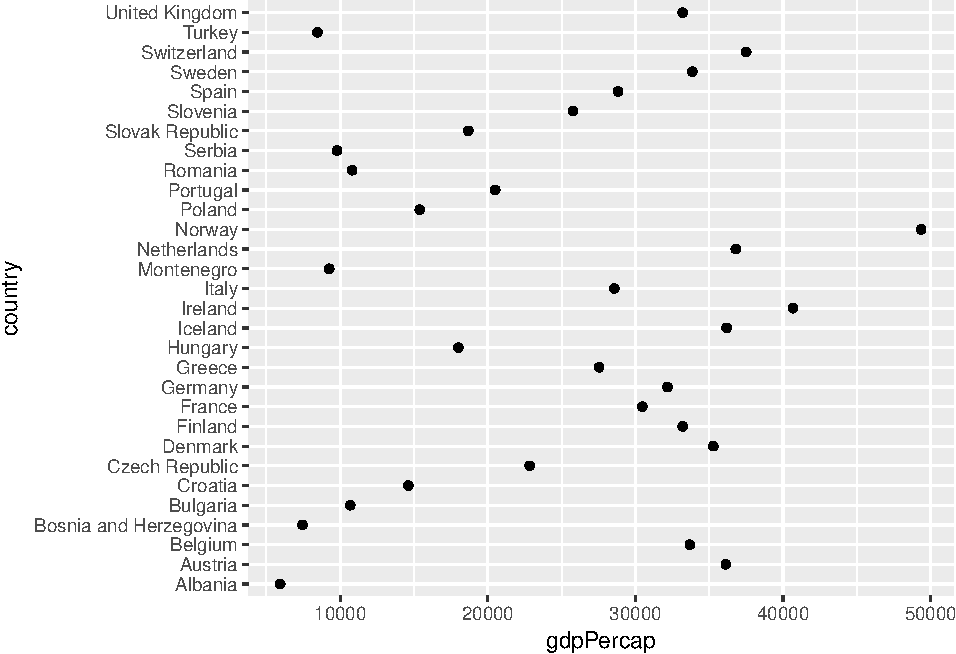
\includegraphics{Intro_graphics_files/figure-latex/plot_eur-1.pdf}

There is high variation---from Albania to Norway.

What about Asian countries in 2007?

\begin{Shaded}
\begin{Highlighting}[]
\NormalTok{data_asia_}\DecValTok{2007}\NormalTok{ <-}\StringTok{ }\NormalTok{data_gapminder }\OperatorTok\StringTok{ }
\StringTok{  }\NormalTok{dplyr}\OperatorTok{::}\KeywordTok{filter}\NormalTok{(year }\OperatorTok{==}\StringTok{ }\DecValTok{2007}\NormalTok{) }\OperatorTok\StringTok{ }\CommentTok{#isolates variables for year 2007}
\StringTok{  }\NormalTok{dplyr}\OperatorTok{::}\KeywordTok{filter}\NormalTok{(continent }\OperatorTok{==}\StringTok{ "Asia"}\NormalTok{) }\CommentTok{#collect only Asian countries}

\NormalTok{(plot_asia <-}\StringTok{ }\KeywordTok{ggplot}\NormalTok{(}\DataTypeTok{data =}\NormalTok{ data_asia_}\DecValTok{2007}\NormalTok{) }\OperatorTok{+}
\StringTok{  }\KeywordTok{geom_point}\NormalTok{(}\DataTypeTok{mapping =} \KeywordTok{aes}\NormalTok{(}\DataTypeTok{x =}\NormalTok{ gdpPercap, }\DataTypeTok{y =}\NormalTok{ country)) }\OperatorTok{+}
\StringTok{  }\KeywordTok{labs}\NormalTok{(}\DataTypeTok{x =} \StringTok{"GDP/capita (USD)"}\NormalTok{, }
       \DataTypeTok{y =} \StringTok{"Country"}\NormalTok{,}
       \DataTypeTok{title =} \StringTok{"GDP per capita in Asia"}\NormalTok{,}
       \DataTypeTok{subtitle =} \StringTok{"Put subtitle here"}\NormalTok{))}
\end{Highlighting}
\end{Shaded}

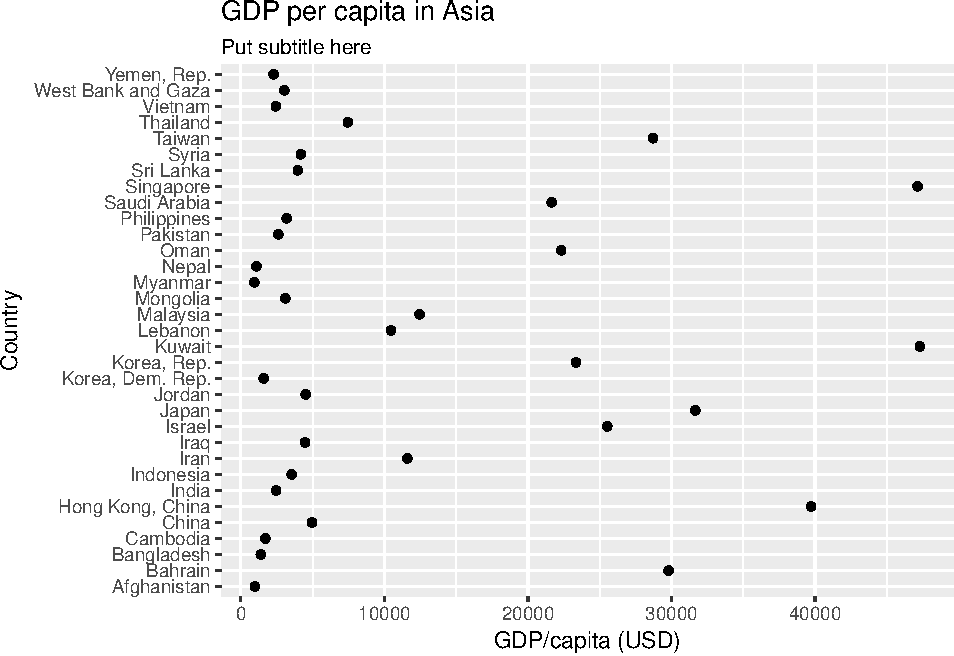
\includegraphics{Intro_graphics_files/figure-latex/plot_asia-1.pdf}

Again, large variation among Asian countries but what about the bounds?
What can we say about the question?

\subsection{Graphics}\label{graphics}

We start with the function \texttt{ggplot()}. It creates a coordinate
system that we will add layers to. The first argument is the dataset to
use in the graph.

\texttt{ggplot(data\ =\ data\_eur\_2007)} creates an empty graph. The
function \texttt{geom\_point()} adds a layer of points to our plot. Each
geom function in ggplot2 takes a mapping argument. This defines how
variables in our dataset are mapped to aesthetics such as axes, colors,
shapes etc. The \(x\) and \(y\) arguments of \texttt{aes()} specify
which variables to map to the \(x\) and \(y\) axes. Variables can also
be mapped to aesthetics such as colors, shapes, sizes etc.

\subsubsection{A More Granular Look: China, India, France,
Germany}\label{a-more-granular-look-china-india-france-germany}

What about life expectancy in these countries with time?

\begin{Shaded}
\begin{Highlighting}[]
\NormalTok{data_CIFG <-}\StringTok{ }\NormalTok{data_gapminder }\OperatorTok
\StringTok{  }\NormalTok{dplyr}\OperatorTok{::}\KeywordTok{filter}\NormalTok{(country }\OperatorTok\StringTok{ }\KeywordTok{c}\NormalTok{(}\StringTok{"China"}\NormalTok{, }
                               \StringTok{"India"}\NormalTok{, }
                               \StringTok{"France"}\NormalTok{, }
                               \StringTok{"Germany"}
\NormalTok{                               )}
\NormalTok{                )}

\NormalTok{(plot_CIFG_life_exp <-}\StringTok{ }\KeywordTok{ggplot}\NormalTok{(}\DataTypeTok{data =}\NormalTok{ data_CIFG) }\OperatorTok{+}
\StringTok{  }\KeywordTok{geom_line}\NormalTok{(}\DataTypeTok{mapping =} \KeywordTok{aes}\NormalTok{(}\DataTypeTok{x =}\NormalTok{ year, }
                          \DataTypeTok{y =}\NormalTok{ lifeExp, }
                          \DataTypeTok{color =}\NormalTok{ country)}
\NormalTok{            )}
\NormalTok{  )}
\end{Highlighting}
\end{Shaded}

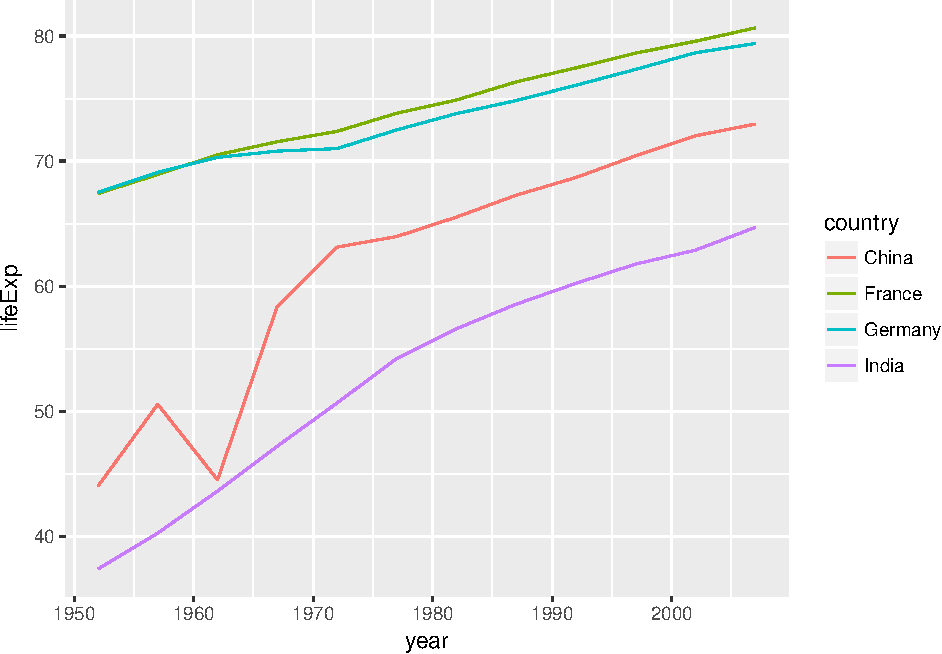
\includegraphics{Intro_graphics_files/figure-latex/CIFG-1.pdf}

\subsubsection{Notes}\label{notes-1}

\begin{enumerate}
\def\labelenumi{\arabic{enumi}.}
\tightlist
\item
  Plots can be stored as variables too.
\item
  Other aesthetic attributes: shape, size, alpha (transparency) etc.
\item
  Note where to put the \texttt{+} sign.
\item
  \texttt{geom\_line()} as opposed to points. Other ``geoms'' are
  \texttt{geom\_smooth}, \texttt{geom\_boxplot}, \texttt{geom\_bar} etc.
\end{enumerate}

\subsubsection{Faceting}\label{faceting}

\begin{Shaded}
\begin{Highlighting}[]
\NormalTok{(plot_CIFG_life_cont <-}\StringTok{ }\KeywordTok{ggplot}\NormalTok{(}\DataTypeTok{data =}\NormalTok{ data_CIFG) }\OperatorTok{+}
\StringTok{  }\KeywordTok{geom_line}\NormalTok{(}\DataTypeTok{mapping =} \KeywordTok{aes}\NormalTok{(}\DataTypeTok{x =}\NormalTok{ year, }
                          \DataTypeTok{y =}\NormalTok{ lifeExp, }
                          \DataTypeTok{color =}\NormalTok{ country)}
\NormalTok{            ) }\OperatorTok{+}
\StringTok{  }\KeywordTok{facet_wrap}\NormalTok{(}\OperatorTok{~}\StringTok{ }\NormalTok{continent)}
\NormalTok{ )}
\end{Highlighting}
\end{Shaded}

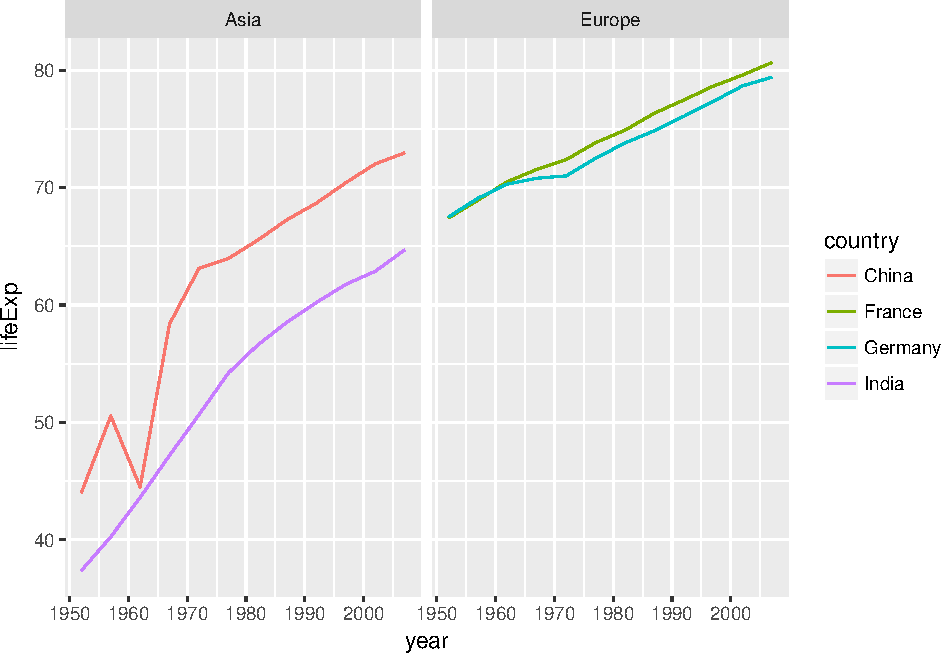
\includegraphics{Intro_graphics_files/figure-latex/CIFG_Facet-1.pdf}

\subsubsection{Notes}\label{notes-2}

\begin{enumerate}
\def\labelenumi{\arabic{enumi}.}
\tightlist
\item
  To facet on one variable (`continent' here), use
  \texttt{facet\_wrap()}.
\item
  To facet on two variables, use \texttt{facet\_grid()}
\end{enumerate}

\subsection{\texorpdfstring{The Notion of Geoms in
\texttt{ggplot()}}{The Notion of Geoms in ggplot()}}\label{the-notion-of-geoms-in-ggplot}

Sometimes one needs bar charts, sometimes histograms; at other times
scatterplots or lines etc. All these are different ``geoms'' in
\texttt{ggplot()}. Scatterplots can be made with \texttt{geom\_point()},
lineplots can be implemented with \texttt{geom\_line()}; boxplots
require \texttt{geom\_boxplot()}, barcharts need \texttt{geom\_bar()}
and so on. Multiple geoms could be part of the same graph. The library
ggplot2 provides over 30 geoms.

Each geom will need ``aesthetic'' parameters: for example, which
datasets form the \(x\) axis? Which ones form the \(y\) axis? What
colors to use for different variables?

Somewhat unsurprisingly, not every aesthetic works with every geom. We
could set the shape parameter of a point, but cannot do so for a line.

This is how we could include multiple geoms in the same plot:

\begin{Shaded}
\begin{Highlighting}[]
\NormalTok{(plot_CIFG_mult_geom <-}\StringTok{ }\KeywordTok{ggplot}\NormalTok{(}\DataTypeTok{data =}\NormalTok{ data_CIFG) }\OperatorTok{+}
\StringTok{   }\KeywordTok{geom_point}\NormalTok{(}\DataTypeTok{mapping =} \KeywordTok{aes}\NormalTok{(}\DataTypeTok{x =}\NormalTok{ year, }\DataTypeTok{y =}\NormalTok{ lifeExp, }\DataTypeTok{color =}\NormalTok{ country)) }\OperatorTok{+}
\StringTok{   }\KeywordTok{geom_line}\NormalTok{(}\DataTypeTok{mapping =} \KeywordTok{aes}\NormalTok{(}\DataTypeTok{x =}\NormalTok{ year, }\DataTypeTok{y =}\NormalTok{ lifeExp, }\DataTypeTok{linetype =}\NormalTok{ country))}
\NormalTok{  )}
\end{Highlighting}
\end{Shaded}

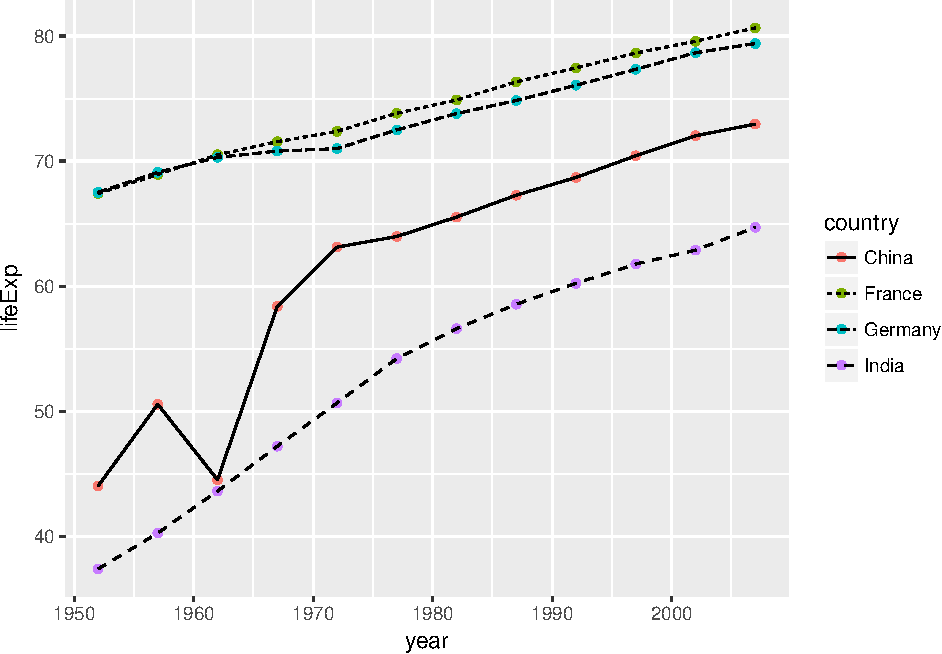
\includegraphics{Intro_graphics_files/figure-latex/CIFG_Mult_Geom-1.pdf}

Note however, that we need to rewrite the code for aesthetic parameters:
\texttt{x\ =\ year,\ y\ =\ lifeExp}. We could re-express the same idea
in fewer lines---by passing some common aesthetic parameters as global
options---by including them in the main \texttt{ggplot} argument:

\begin{Shaded}
\begin{Highlighting}[]
\NormalTok{plot_CIFG_mult_geom_}\DecValTok{2}\NormalTok{ <-}\StringTok{ }\KeywordTok{ggplot}\NormalTok{(}\DataTypeTok{data =}\NormalTok{ data_CIFG, }
                                \DataTypeTok{mapping =} \KeywordTok{aes}\NormalTok{(}\DataTypeTok{x =}\NormalTok{ year, }
                                              \DataTypeTok{y =}\NormalTok{ lifeExp)) }\OperatorTok{+}
\StringTok{  }\KeywordTok{geom_point}\NormalTok{(}\DataTypeTok{mapping =}  \KeywordTok{aes}\NormalTok{(}\DataTypeTok{color =}\NormalTok{ country)) }\OperatorTok{+}
\StringTok{  }\KeywordTok{geom_line}\NormalTok{(}\DataTypeTok{mapping =} \KeywordTok{aes}\NormalTok{(}\DataTypeTok{linetype =}\NormalTok{ country))}
\end{Highlighting}
\end{Shaded}

\subsubsection{\texorpdfstring{Plotting linear trends:
\texttt{geom\_smooth()}}{Plotting linear trends: geom\_smooth()}}\label{plotting-linear-trends-geom_smooth}

Fitting a line to a set of observations is linear smoothing. Fitting a
polynomial of degree 2 is quadratic smoothing and so on. When we wish to
plot observations and the best linear fit computed by linear regression,
we need to use \texttt{geom\_smooth()} with the option
\texttt{method\ =\ "lm"} where \texttt{lm()} stands for ``linear
model''.

\subsubsection{Question: What was population growth in
India?}\label{question-what-was-population-growth-in-india}

\begin{Shaded}
\begin{Highlighting}[]
\NormalTok{(plot_CIFG_pop_Ind <-}\StringTok{ }\KeywordTok{ggplot}\NormalTok{(}\DataTypeTok{data =} \KeywordTok{filter}\NormalTok{(data_CIFG, }\CommentTok{#why no +?}
\NormalTok{                                           country }\OperatorTok{==}\StringTok{ "India"}\NormalTok{), }
                         \DataTypeTok{mapping =} \KeywordTok{aes}\NormalTok{(}\DataTypeTok{x =}\NormalTok{ year, }\DataTypeTok{y =}\NormalTok{ pop)) }\OperatorTok{+}
\StringTok{  }\KeywordTok{geom_point}\NormalTok{(}\DataTypeTok{mapping =} \KeywordTok{aes}\NormalTok{(}\DataTypeTok{color =}\NormalTok{ country)) }\OperatorTok{+}
\StringTok{  }\KeywordTok{geom_smooth}\NormalTok{(}\DataTypeTok{method =} \StringTok{"lm"}\NormalTok{, }\DataTypeTok{se =}\NormalTok{ F) }\CommentTok{#se = "standard errors"}
\NormalTok{ )}
\end{Highlighting}
\end{Shaded}

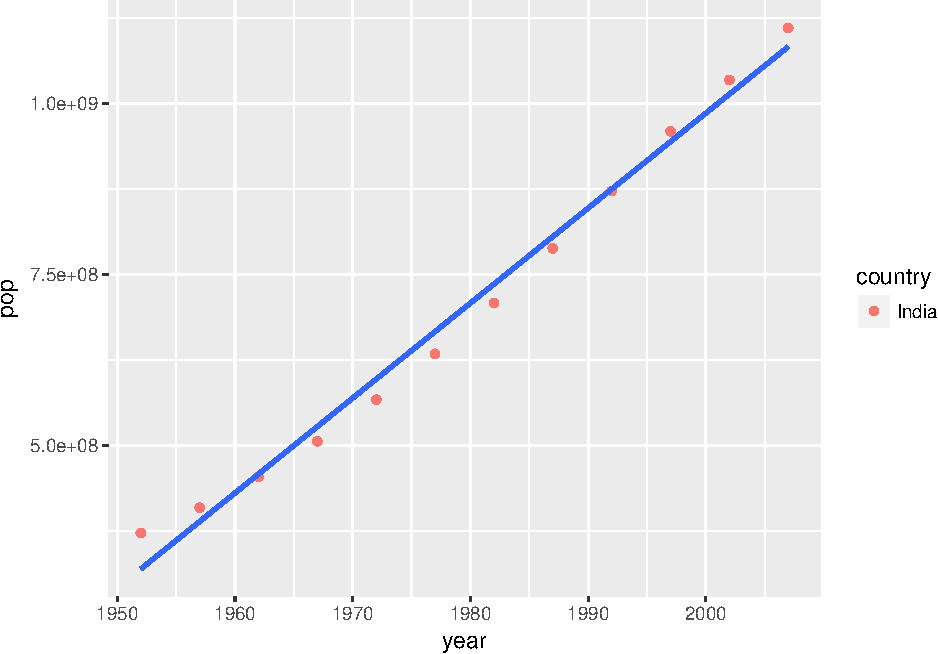
\includegraphics{Intro_graphics_files/figure-latex/CIFG_pop_Ind-1.pdf}

\subsubsection{Question: What about the same in
China?}\label{question-what-about-the-same-in-china}

\begin{Shaded}
\begin{Highlighting}[]
\NormalTok{(plot_CIFG_pop_China <-}\StringTok{ }\KeywordTok{ggplot}\NormalTok{(}\DataTypeTok{data =} \KeywordTok{filter}\NormalTok{(data_CIFG, }
\NormalTok{                                             country }\OperatorTok{==}\StringTok{ "China"}\NormalTok{), }
                         \DataTypeTok{mapping =} \KeywordTok{aes}\NormalTok{(}\DataTypeTok{x =}\NormalTok{ year, }\DataTypeTok{y =}\NormalTok{ pop)) }\OperatorTok{+}
\StringTok{  }\KeywordTok{geom_point}\NormalTok{(}\DataTypeTok{mapping =} \KeywordTok{aes}\NormalTok{(}\DataTypeTok{color =}\NormalTok{ country)) }\OperatorTok{+}
\StringTok{  }\KeywordTok{geom_smooth}\NormalTok{(}\DataTypeTok{method =} \StringTok{"lm"}\NormalTok{) }\CommentTok{#se = T by default}
\NormalTok{ )}
\end{Highlighting}
\end{Shaded}

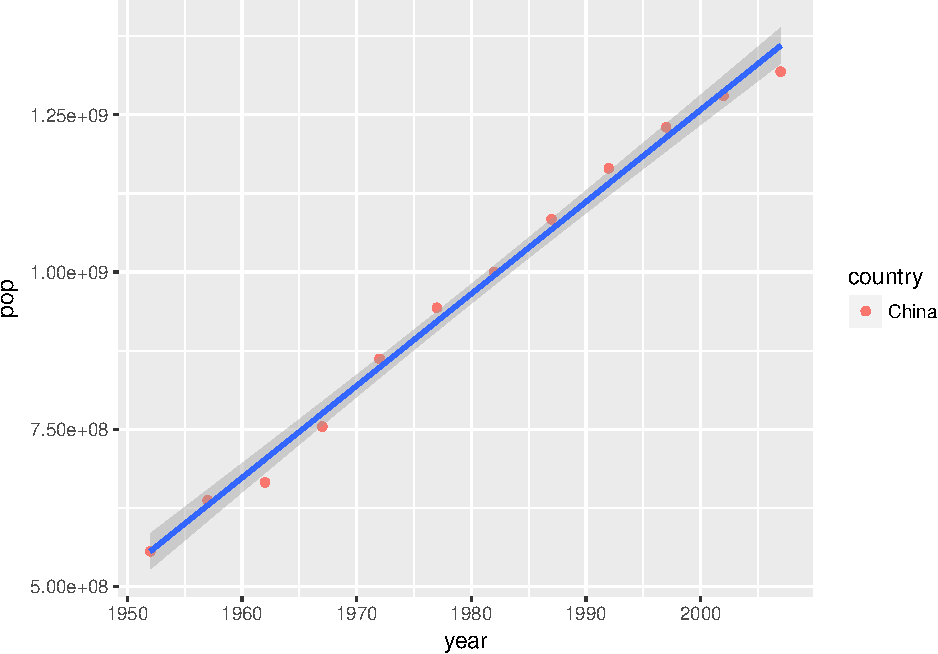
\includegraphics{Intro_graphics_files/figure-latex/CIFG_pop_China-1.pdf}

The default smoothing method however is ``loess'' (locally weighted
scatterplot smoothing)

\begin{Shaded}
\begin{Highlighting}[]
\NormalTok{(plot_CIFG_pop_Ind <-}\StringTok{ }\KeywordTok{ggplot}\NormalTok{(}\DataTypeTok{data =} \KeywordTok{filter}\NormalTok{(data_CIFG, }
\NormalTok{                                           continent }\OperatorTok{==}\StringTok{ "Asia"}\NormalTok{), }
                         \DataTypeTok{mapping =} \KeywordTok{aes}\NormalTok{(}\DataTypeTok{x =}\NormalTok{ year, }\DataTypeTok{y =}\NormalTok{ pop)) }\OperatorTok{+}
\StringTok{  }\KeywordTok{geom_point}\NormalTok{(}\DataTypeTok{mapping =} \KeywordTok{aes}\NormalTok{(}\DataTypeTok{color =}\NormalTok{ country)) }\OperatorTok{+}
\StringTok{  }\KeywordTok{geom_smooth}\NormalTok{() }
\NormalTok{ )}
\end{Highlighting}
\end{Shaded}

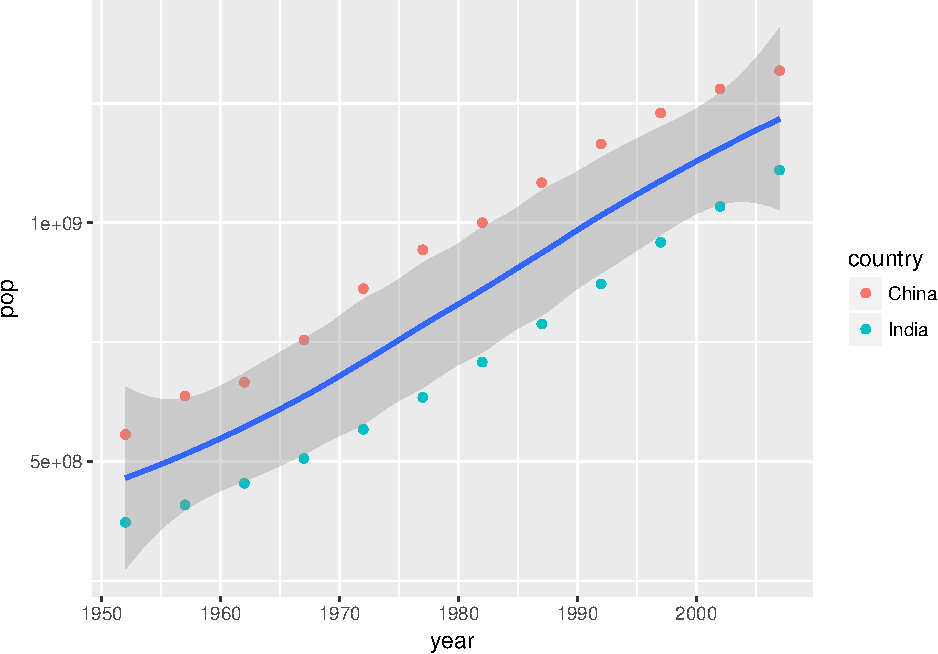
\includegraphics{Intro_graphics_files/figure-latex/CIFG_pop_Asia_loess-1.pdf}

\subsection{Bar Charts}\label{bar-charts}

What about GDP per capita of CIFG countries in 2007?

\begin{Shaded}
\begin{Highlighting}[]
\NormalTok{(plot_CIFG_pop_}\DecValTok{2007}\NormalTok{ <-}\StringTok{ }\KeywordTok{ggplot}\NormalTok{(}\DataTypeTok{data =} \KeywordTok{filter}\NormalTok{(data_CIFG,}
\NormalTok{                                            year }\OperatorTok{==}\StringTok{ }\DecValTok{2007}\NormalTok{),}
                              \DataTypeTok{mapping =} \KeywordTok{aes}\NormalTok{(}\DataTypeTok{x =}\NormalTok{ country, }
                                            \DataTypeTok{y =}\NormalTok{ gdpPercap)) }\OperatorTok{+}\StringTok{ }
\StringTok{   }\KeywordTok{geom_bar}\NormalTok{(}\DataTypeTok{mapping =} \KeywordTok{aes}\NormalTok{(}\DataTypeTok{fill =}\NormalTok{ country), }\CommentTok{#what does this mean?}
            \DataTypeTok{stat =} \StringTok{"identity"}\NormalTok{) }\CommentTok{#what does this mean?}
\NormalTok{ )}
\end{Highlighting}
\end{Shaded}

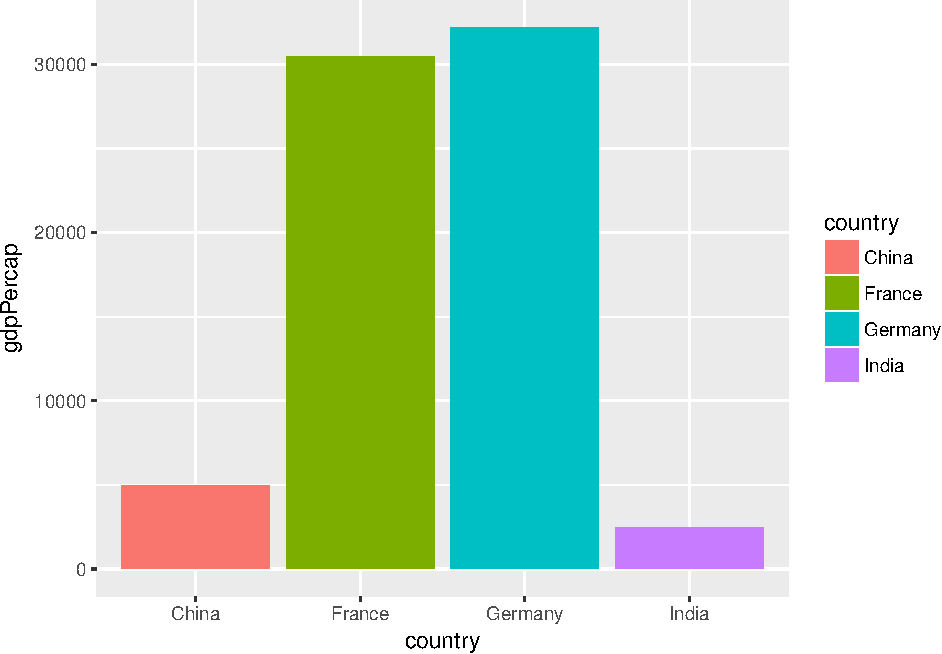
\includegraphics{Intro_graphics_files/figure-latex/CIFG_pop_2007-1.pdf}

While some types of plots (scatterplots) do not require any
transformation---each point is plotted at \(x\) and \(y\) coordinates
same as the original value, others (such as boxplots, histograms etc.)
require transformations. For example, for boxplots, the median and the
interquartile range (IQR) need computing.

\subsection{Boxplots}\label{boxplots}

\begin{Shaded}
\begin{Highlighting}[]
\NormalTok{(plot_CIFG_box <-}\StringTok{ }\KeywordTok{ggplot}\NormalTok{(}\DataTypeTok{data =}\NormalTok{ data_CIFG,}
                         \DataTypeTok{mapping =} \KeywordTok{aes}\NormalTok{(}\DataTypeTok{x =}\NormalTok{ country, }
                                       \DataTypeTok{y =}\NormalTok{ lifeExp,}
                                       \DataTypeTok{color =}\NormalTok{ country)) }\OperatorTok{+}
\StringTok{   }\KeywordTok{geom_boxplot}\NormalTok{()}
\NormalTok{   )}
\end{Highlighting}
\end{Shaded}

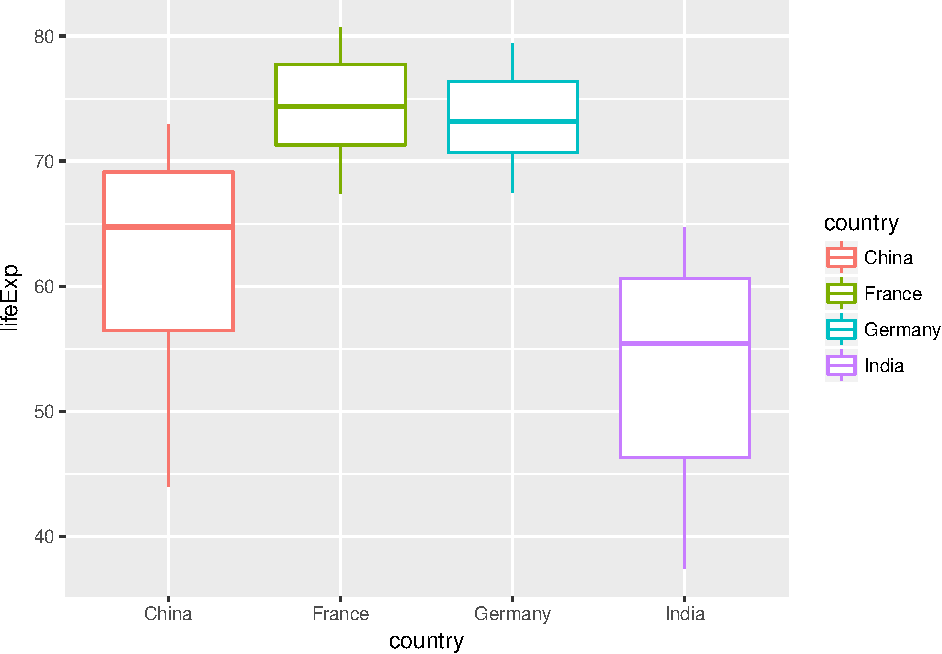
\includegraphics{Intro_graphics_files/figure-latex/plot_CIFG_box-1.pdf}

In some cases there are many variables for which we need boxplots; and
including all of them on the \(x\) axis may cause their names to squish
together, leading to poor visibility. In such cases, one can use the
command \texttt{coord\_flip()} which, as the name suggests, flips the
coordinates---from \(x\) to \(y\) and vice versa.

\begin{Shaded}
\begin{Highlighting}[]
\NormalTok{(plot_eur_box_flip <-}\StringTok{ }\KeywordTok{ggplot}\NormalTok{(}\DataTypeTok{data =} \KeywordTok{filter}\NormalTok{(data_gapminder,}
\NormalTok{                                           continent }\OperatorTok{==}\StringTok{ "Europe"}\NormalTok{),}
                         \DataTypeTok{mapping =} \KeywordTok{aes}\NormalTok{(}\DataTypeTok{x =}\NormalTok{ country, }
                                       \DataTypeTok{y =}\NormalTok{ lifeExp,}
                                       \DataTypeTok{color =}\NormalTok{ country)) }\OperatorTok{+}
\StringTok{   }\KeywordTok{geom_boxplot}\NormalTok{() }\OperatorTok{+}
\StringTok{   }\KeywordTok{coord_flip}\NormalTok{()}
\NormalTok{   )}
\end{Highlighting}
\end{Shaded}

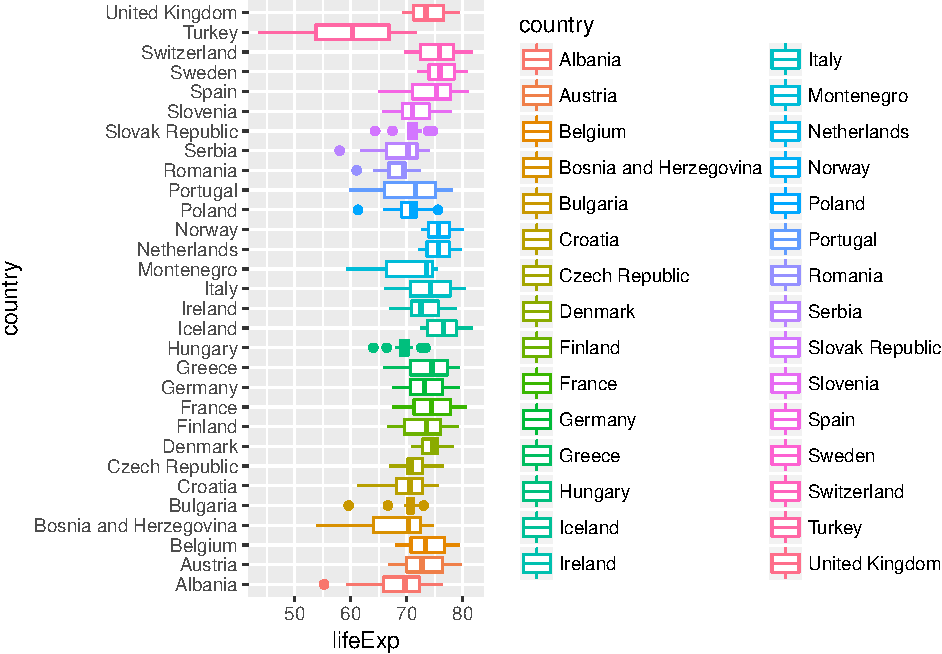
\includegraphics{Intro_graphics_files/figure-latex/plot_eur_box_flip-1.pdf}

\subsection{Themes}\label{themes}

Themes govern the overall ``look'' of the plot. The default theme is
\texttt{theme\_grey()}. However, there are dozens of other themes which
one may prefer. A small set of examples is presented here.

\begin{Shaded}
\begin{Highlighting}[]
\NormalTok{(plot_CIFG_theme <-}\StringTok{ }\KeywordTok{ggplot}\NormalTok{(}\DataTypeTok{data =}\NormalTok{ data_CIFG, }
                                \DataTypeTok{mapping =} \KeywordTok{aes}\NormalTok{(}\DataTypeTok{x =}\NormalTok{ year, }
                                              \DataTypeTok{y =}\NormalTok{ lifeExp)) }\OperatorTok{+}
\StringTok{  }\KeywordTok{geom_point}\NormalTok{(}\DataTypeTok{mapping =}  \KeywordTok{aes}\NormalTok{(}\DataTypeTok{color =}\NormalTok{ country)) }\OperatorTok{+}
\StringTok{  }\KeywordTok{geom_line}\NormalTok{(}\DataTypeTok{mapping =} \KeywordTok{aes}\NormalTok{(}\DataTypeTok{linetype =}\NormalTok{ country)) }\OperatorTok{+}
\StringTok{   }\KeywordTok{labs}\NormalTok{(}\DataTypeTok{x =} \StringTok{"Years"}\NormalTok{, }
        \DataTypeTok{y =} \StringTok{"Life Expectancy"}\NormalTok{,}
        \DataTypeTok{title =} \StringTok{"Illustration of Different Themes"}\NormalTok{) }\OperatorTok{+}
\StringTok{  }\KeywordTok{theme_classic}\NormalTok{() }\CommentTok{#note the classic theme}
\NormalTok{ )}
\end{Highlighting}
\end{Shaded}

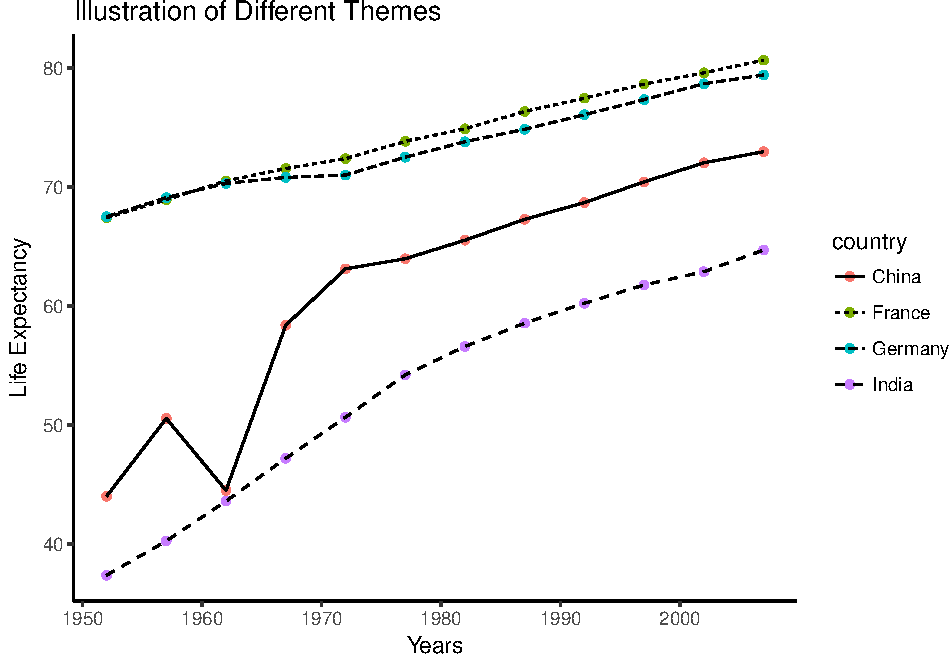
\includegraphics{Intro_graphics_files/figure-latex/CIFG_theme-1.pdf}

\begin{Shaded}
\begin{Highlighting}[]
\NormalTok{(plot_CIFG_theme <-}\StringTok{ }\KeywordTok{ggplot}\NormalTok{(}\DataTypeTok{data =}\NormalTok{ data_CIFG, }
                                \DataTypeTok{mapping =} \KeywordTok{aes}\NormalTok{(}\DataTypeTok{x =}\NormalTok{ year, }
                                              \DataTypeTok{y =}\NormalTok{ lifeExp)) }\OperatorTok{+}
\StringTok{  }\KeywordTok{geom_point}\NormalTok{(}\DataTypeTok{mapping =}  \KeywordTok{aes}\NormalTok{(}\DataTypeTok{color =}\NormalTok{ country)) }\OperatorTok{+}
\StringTok{  }\KeywordTok{geom_line}\NormalTok{(}\DataTypeTok{mapping =} \KeywordTok{aes}\NormalTok{(}\DataTypeTok{linetype =}\NormalTok{ country)) }\OperatorTok{+}
\StringTok{   }\KeywordTok{labs}\NormalTok{(}\DataTypeTok{x =} \StringTok{"Years"}\NormalTok{, }
        \DataTypeTok{y =} \StringTok{"Life Expectancy"}\NormalTok{,}
        \DataTypeTok{title =} \StringTok{"Illustration of Different Themes"}\NormalTok{) }\OperatorTok{+}
\StringTok{  }\KeywordTok{theme_bw}\NormalTok{() }\CommentTok{#note the bw theme (black and white)}
\NormalTok{ )}
\end{Highlighting}
\end{Shaded}

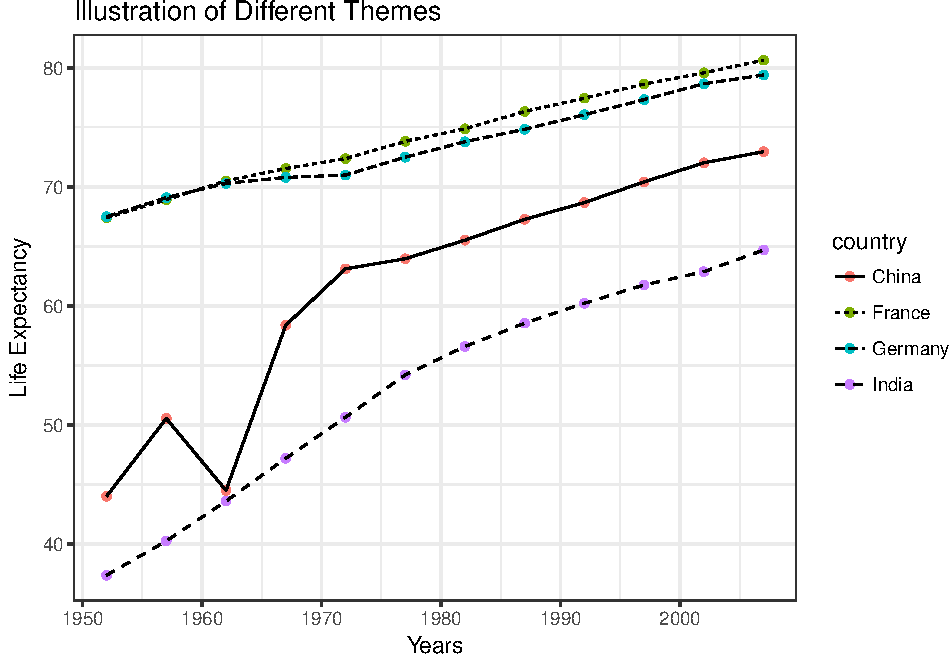
\includegraphics{Intro_graphics_files/figure-latex/CIFG_theme-2.pdf}

\begin{Shaded}
\begin{Highlighting}[]
\NormalTok{(plot_CIFG_theme <-}\StringTok{ }\KeywordTok{ggplot}\NormalTok{(}\DataTypeTok{data =}\NormalTok{ data_CIFG, }
                                \DataTypeTok{mapping =} \KeywordTok{aes}\NormalTok{(}\DataTypeTok{x =}\NormalTok{ year, }
                                              \DataTypeTok{y =}\NormalTok{ lifeExp)) }\OperatorTok{+}
\StringTok{  }\KeywordTok{geom_point}\NormalTok{(}\DataTypeTok{mapping =}  \KeywordTok{aes}\NormalTok{(}\DataTypeTok{color =}\NormalTok{ country)) }\OperatorTok{+}
\StringTok{  }\KeywordTok{geom_line}\NormalTok{(}\DataTypeTok{mapping =} \KeywordTok{aes}\NormalTok{(}\DataTypeTok{linetype =}\NormalTok{ country)) }\OperatorTok{+}
\StringTok{   }\KeywordTok{labs}\NormalTok{(}\DataTypeTok{x =} \StringTok{"Years"}\NormalTok{, }
        \DataTypeTok{y =} \StringTok{"Life Expectancy"}\NormalTok{,}
        \DataTypeTok{caption =} \StringTok{"Insert caption here"}\NormalTok{,}
        \DataTypeTok{title =} \StringTok{"Illustration of Different Themes"}\NormalTok{) }\OperatorTok{+}
\StringTok{  }\KeywordTok{theme_minimal}\NormalTok{() }\CommentTok{#note the minimal theme}
\NormalTok{ )}
\end{Highlighting}
\end{Shaded}

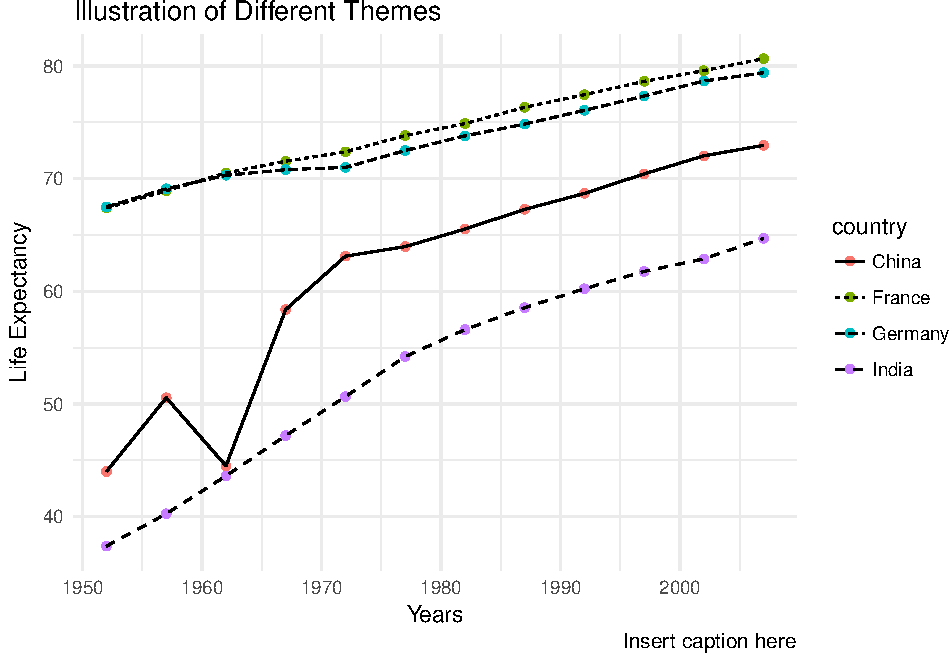
\includegraphics{Intro_graphics_files/figure-latex/CIFG_theme-3.pdf}

\section{FAQ: How to Plot Multiple Variables
Together?}\label{faq-how-to-plot-multiple-variables-together}

\subsection{Wide Versus Long Data}\label{wide-versus-long-data}

When each column is a separate variable, the dataset is said to be in
the ``wide'' format. In the ``long'' format, variables are ``gathered''
together in one column with another containing values.

\begin{Shaded}
\begin{Highlighting}[]
\NormalTok{temp_w <-}\StringTok{ }\KeywordTok{cbind}\NormalTok{(}\DecValTok{1991}\OperatorTok{:}\DecValTok{2010}\NormalTok{, }
                \KeywordTok{rnorm}\NormalTok{(}\DecValTok{20}\NormalTok{, }\DecValTok{0}\NormalTok{, }\DecValTok{1}\NormalTok{), }
                \KeywordTok{rnorm}\NormalTok{(}\DecValTok{20}\NormalTok{, }\DecValTok{2}\NormalTok{, }\DecValTok{5}\NormalTok{),}
                \KeywordTok{rnorm}\NormalTok{(}\DecValTok{20}\NormalTok{, }\DecValTok{1}\NormalTok{, }\DecValTok{9}\NormalTok{)) }\OperatorTok
\StringTok{  }\NormalTok{tibble}\OperatorTok{::}\KeywordTok{as_tibble}\NormalTok{()}
\KeywordTok{names}\NormalTok{(temp_w) <-}\StringTok{ }\KeywordTok{c}\NormalTok{(}\StringTok{"year"}\NormalTok{, }\StringTok{"N01"}\NormalTok{, }\StringTok{"N25"}\NormalTok{, }\StringTok{"N19"}\NormalTok{) }\CommentTok{#data in "wide" format}

\KeywordTok{head}\NormalTok{(temp_w)}
\end{Highlighting}
\end{Shaded}

\begin{verbatim}
## # A tibble: 6 x 4
##    year     N01    N25    N19
##   <dbl>   <dbl>  <dbl>  <dbl>
## 1  1991  1.50   -3.05   -9.00
## 2  1992 -0.645   6.32   11.6 
## 3  1993 -1.42    5.89    2.80
## 4  1994  0.676  -7.57   -6.66
## 5  1995  0.772   4.93   -2.93
## 6  1996  0.0370  0.962  -8.99
\end{verbatim}

\begin{Shaded}
\begin{Highlighting}[]
\NormalTok{(}\KeywordTok{ggplot}\NormalTok{(}\DataTypeTok{data =}\NormalTok{ temp_w,}
        \DataTypeTok{mapping =} \KeywordTok{aes}\NormalTok{(}\DataTypeTok{x =}\NormalTok{ year)) }\OperatorTok{+}\StringTok{ }
\StringTok{    }\KeywordTok{geom_line}\NormalTok{(}\DataTypeTok{mapping =} \KeywordTok{aes}\NormalTok{(}\DataTypeTok{y =}\NormalTok{ N01), }\DataTypeTok{color =} \StringTok{"red"}\NormalTok{) }\OperatorTok{+}
\StringTok{    }\KeywordTok{geom_line}\NormalTok{(}\DataTypeTok{mapping =} \KeywordTok{aes}\NormalTok{(}\DataTypeTok{y =}\NormalTok{ N25), }\DataTypeTok{color =} \StringTok{"blue"}\NormalTok{) }\OperatorTok{+}
\StringTok{    }\KeywordTok{geom_line}\NormalTok{(}\DataTypeTok{mapping =} \KeywordTok{aes}\NormalTok{(}\DataTypeTok{y =}\NormalTok{ N19), }\DataTypeTok{color =} \StringTok{"green"}\NormalTok{)}
\NormalTok{  ) }\CommentTok{#this method of plotting is not encouraged}
\end{Highlighting}
\end{Shaded}

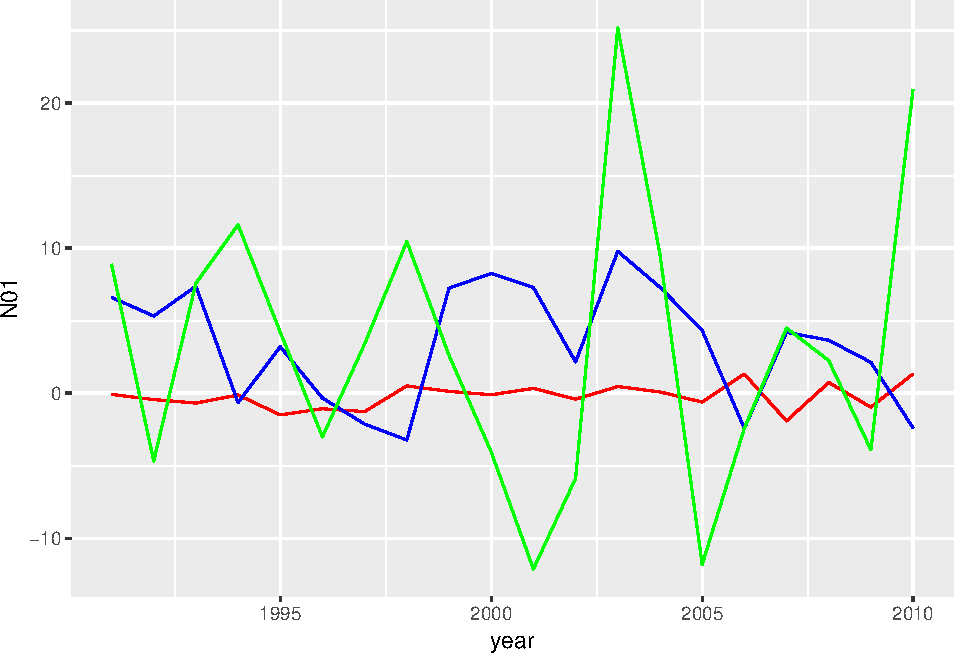
\includegraphics{Intro_graphics_files/figure-latex/wide_vs_long-1.pdf}

\begin{Shaded}
\begin{Highlighting}[]
\NormalTok{temp_l <-}\StringTok{ }\NormalTok{tidyr}\OperatorTok{::}\KeywordTok{gather}\NormalTok{(temp_w, }\KeywordTok{c}\NormalTok{(}\StringTok{"N01"}\NormalTok{, }\StringTok{"N25"}\NormalTok{, }\StringTok{"N19"}\NormalTok{), }
                        \DataTypeTok{key =} \StringTok{"Normal RV"}\NormalTok{, }
                        \DataTypeTok{value =} \StringTok{"Normal Realization"}
\NormalTok{                        ) }\CommentTok{#converting data from wide to "long"}

\KeywordTok{head}\NormalTok{(temp_l)}
\end{Highlighting}
\end{Shaded}

\begin{verbatim}
## # A tibble: 6 x 3
##    year `Normal RV` `Normal Realization`
##   <dbl> <chr>                      <dbl>
## 1  1991 N01                       1.50  
## 2  1992 N01                      -0.645 
## 3  1993 N01                      -1.42  
## 4  1994 N01                       0.676 
## 5  1995 N01                       0.772 
## 6  1996 N01                       0.0370
\end{verbatim}

\begin{Shaded}
\begin{Highlighting}[]
\NormalTok{(}\KeywordTok{ggplot}\NormalTok{(}\DataTypeTok{data =}\NormalTok{ temp_l,}
        \DataTypeTok{mapping =} \KeywordTok{aes}\NormalTok{(}\DataTypeTok{x =}\NormalTok{ year, }
                      \DataTypeTok{y =} \StringTok{`}\DataTypeTok{Normal Realization}\StringTok{`}\NormalTok{,}
                      \DataTypeTok{color =} \StringTok{`}\DataTypeTok{Normal RV}\StringTok{`}\NormalTok{)) }\OperatorTok{+}
\StringTok{    }\KeywordTok{geom_line}\NormalTok{()}
\NormalTok{  ) }\CommentTok{#the preferred way of plotting is in the long format}
\end{Highlighting}
\end{Shaded}

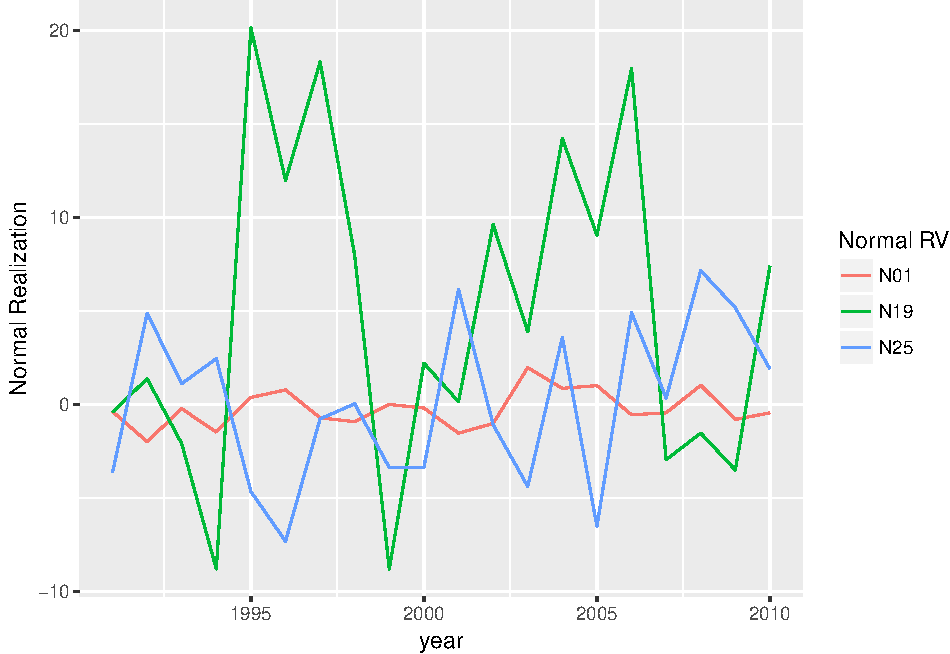
\includegraphics{Intro_graphics_files/figure-latex/wide_vs_long-2.pdf}

\section*{References}\label{references}
\addcontentsline{toc}{section}{References}

\hypertarget{refs}{}
\hypertarget{ref-Wickham:2010}{}
Wickham, Hadley. 2010. ``A Layered Grammar of Graphics.'' \emph{Journal
of Computational and Graphical Statistics} 19 (1): 3--28.

\hypertarget{ref-Wilkinson:2005}{}
Wilkinson, Leland. 2005. \emph{The Grammar of Graphics (Statistics and
Computing)}. Berlin, Heidelberg: Springer-Verlag.


\end{document}
